\documentclass[numbers=noenddot]{thesis}

% hier namen etc. einsetzen
\fullname{Fabian Fischbach, Luis Beaucamp und Tim Stenzel}
%\email{vorname.nachname@uni-ulm.de}
\headline{Mobile Application Lab}
\titel{Thema}
\jahr{2017}
\matnr{Matrikel-Nr}
\gutachterA{Marc Schickler}
%\gutachterB{Gutachter 2}
\betreuer{Marc Schickler}
\typ{Ausarbeitung zur App }
\fakultaet{Ingenieurwissenschaften, Informatik und \\Psychologie}
\institut{Institut für Datenbanken und Informationssysteme}

% Falls keine Lizenz gewünscht wird bitte den folgenden Text entfernen.
% Die Lizenz erlaubt es zu nichtkommerziellen Zwecken die Arbeit zu
% vervielfältigen und Kopien zu machen. Dabei muss aber immer der Autor
% angegeben werden. Eine kommerzielle Verwertung ist für den Autor
% weiter möglich.
\license{
This work is licensed under the Creative Commons.
Attribution-NonCommercial-ShareAlike 3.0 License. To view a copy of this
license, visit http://creativecommons.org/licenses/by-nc-sa/3.0/de/ or send a
letter to Creative Commons, 543 Howard Street, 5th Floor, San Francisco,
California, 94105, USA. \\ Satz: PDF-\LaTeXe
}

\hypersetup{%
	pdftitle=\pdfescapestring{\thetitel},
	pdfauthor={\thefullname},
 	pdfsubject={\thetyp},
}


% trennungsregeln
\hyphenation{Sil-ben-trenn-ung}

\begin{document}
\frontmatter
\maketitle
% impressum
\clearpage
\impressum

\cleardoublepage
% ab hier zeilenabstand 1,4 fach 10pt/14pt
\setstretch{1.4}

%\section*{Kurzfassung}
Die Kurzfassung (engl. Abstract) einer Abschlussarbeit enthält zwei Blöcke. Der
erste Block enthält eine  kurze Hinführung/Motivation zum Thema sowie einer
anschließenden Beschreibung der Problemstellung (ca. 5-8 Sätze). Der zweite
Block der Kursfassung gibt die Zielsetzung bzw. den Beitrag der Abschlussarbeit
wieder (ebenfalls ca. 5-8 Sätze).

===========================================

ChangeLog:

2015-10-12: Hacks für Literaturverzeichnis eingebaut. Kommentare in der BibTex
Datei beachten!

2015-07-21: Fakultätname angepasst (+ Psychologie)



%\cleardoublepage
%\section*{Danksagung}
An dieser Stelle erfolgt die Danksagung an Personen, die einen bei der Erstellung der Abschlussarbeit unterstützt haben.

% inhaltsverzeichnis einfügen
\tableofcontents

\mainmatter
% hier kommen die kapitel der arbeit
\chapter{Einleitung}
\label{cha:einleitung}

In dieser Dokumentation wird die Entwicklung einer Quartett-App im Rahmen des Anwendungsfaches ``Mobile Application Lab'' an der Universität Ulm vorgestellt und die dabei entwickelte Anwendung präsentiert.

% Abschnitt: Problemstellung
\section{Motivation und Problemstellung}
\label{sec:einleitung:problemstellung}

Die Problemstellung wurde uns im Rahmen dieses Projektes schon gegeben, da wir uns auf die Entwicklung einer Quartett-App für Smartphones konzentrieren sollten. Das beliebte Kartenspiel soll für ein Smartphone umgesetzt werden und so zu jeder Zeit und an jedem Ort auch komplett ohne physische Karten spielbar sein.

Beim Betrachten des aktuellen Marktes für Quartett-Apps fällt schnell die Vielzahl an verschiedenen Apps auf. Diese weisen nach genauerer Untersuchung jedoch teilweise erhebliche Mängel auf. So sind manche von ihnen sehr veraltet und funktionieren nicht mehr richtig auf neueren Smartphone-Modellen. Auch entsprechen diese inhaltlich nicht unseren Vorstellungen einer guten Quartett-App. Sie sind sehr beschränkt, was die verschiedenen Spielmodi angeht, und enthalten meist nur ein einziges Kartendeck oder nur Decks aus einem bestimmten Themengebiet. In diesem Punkt wollen wir uns von den existierenden Apps absetzen.

% Abschnitt: Zielsetzung
\section{Zielsetzung}
\label{sec:einleitung:zielsetzung}

Wir wollen also die Nachfrage des Marktes ausnutzen und eine eigene Quartett-Anwendung erstellen. Diese wollen wir auf Basis von Android und Java entwickeln. Dabei geht es uns primär darum, den Umgang mit den neuen Techniken zu erlernen und Erfahrung im Programmieren von Android-Anwendungen zu erlangen, sodass wir diese nach Abschluss des Projektes beherrschen.

Inhaltlich möchten wir eine Quartett-App entwickeln, die sich im Einzelspielermodus wie ein richtiges Quartett spielen lässt. Sie soll verschiedene Spielmodi haben, welche frei konfigurierbar sein sollen. Zudem soll die App nicht auf ein Deck oder einen Themenbereich beschränkt sein. Dies soll durch einen ``Deckcreator'' und eine Funktion zum hoch- und herunterladen von Decks realisiert werden. Die Anwendung soll zudem die Möglichkeit bieten, alle Karten anzugucken sowie laufende Spiele zu unterbrechen. Dabei soll die App benutzerfreundlich sein und schön aussehen, sowie auf dem Großteil der momentan verwendeten Android-Versionen lauffähig sein.

% Abschnitt: Struktur der Arbeit
\section{Struktur der Arbeit}
\label{sec:einleitung:struktur}

In dieser Dokumentation werden zuerst die grundlegenden Quartett-Spielregeln erklärt, das Betriebssystem Android vorgestellt, sowie unsere verwendeten Frameworks präsentiert. Den Hauptteil bildet das Kapitel über die Implementierung, worin unsere App im Allgemeinen und mit ihren Besonderheiten vorstellt wird. Außerdem wird darin unsere Architektur gezeigt und auf Schwierigkeiten eingegangen, die während der Implementierungsphase auftraten. Darauf folgt ein Abgleich der Anforderungen mit der tatsächlichen Implementierung, und schließlich eine Zusammenfassung und ein Ausblick auf die Zukunft des Projektes.\\

\begin{figure}[htp]
	\centering
  	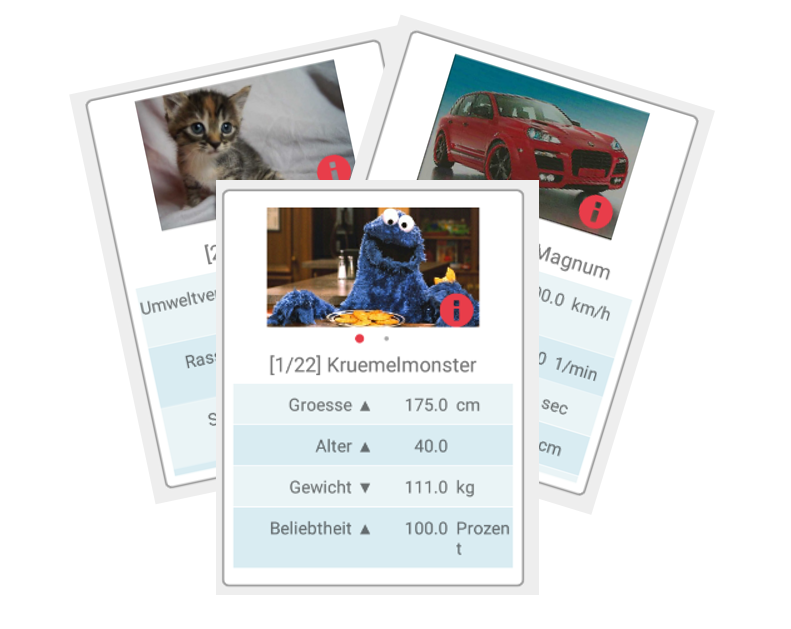
\includegraphics[width=0.4\textwidth]{img/quartett42_logo.png}
	\caption{Quartett42 Logo}
	\label{figure:quartett42logo}
\end{figure}

\chapter{Grundlagen}
\label{cha:grundlagen}

% Abschnitt: Quartettspiel
\section{Quartettspiel}
\label{sec:grundlagen:quartettspiel}

Zum Quartettspielen sind natürlich einige Regeln notwendig, die im Folgenden erklärt werden. \\
Gespielt wird Eins gegen Eins, Spieler gegen Computer. Zuerst wählt der Spieler den Schwierigkeitsgrad (leicht, mittel oder schwer) des Computers, dann den Spielmodus und das Limit für das Spielende (Zeit-, Runden- oder Punktemodus und entsprechend die Spielzeit, Runden- oder Punkteanzahl). Danach wird ein Deck gewählt und gemischt. Computer und Spieler bekommen jeweils die Hälfte der Karten verdeckt auf einem Stapel, bei dem immer nur die oberste Karte sichtbar ist, und es wird zufällig bestimmt wer mit dem ersten Zug beginnen darf. Ein Zug läuft im Grunde genauso ab wie beim ``echten'' Quartett: Der Spieler, der am Zug ist, wählt ein Attribut (Beispiel in einem Autoquartett: Höchstgeschwindigkeit) und nennt den entsprechenden Wert. Der andere Spieler gibt nun ebenfalls seinen Wert bei dem gewählten Attribut bekannt (Beispiel von oben: Höchstgeschwindigkeit) und die Werte werden verglichen. Für jedes Attribut wurde vor dem Spiel festgelegt ob für dieses ein höherer oder niedrigerer Wert gewinnt. Darauf basierend wird nun der Vergleich durchgeführt. Der Spieler mit dem besseren Wert gewinnt den Vergleich, bekommt beide Karten unter seinen Stapel und darf im nächsten Vergleich das Attribut wählen. Bei einem Unentschieden behält jeder seine Karte, legt sie unter seinen Stapel und der Spieler, der das Attribut gewählt hat, wählt auch das nächste. Das Spiel ist zu Ende, wenn ein Spieler keine Karten mehr auf seinem Stapel hat, oder wenn das Limit des gewählten Spielmodus erreicht ist (Zeit abgelaufen / alle Runden ausgespielt / Punktelimit erreicht).

Dies sind die normalen Regeln und Spielmodi für ein Quartettspiel. In unserer App gibt es aber zusätzlich neben dem normalen Modus (bei dem jeweils, wie festgelegt, der höhere oder niedrigere Wert den Vergleich gewinnt) auch noch den sog. ``Insane-Modus'', bei dem jeweils nicht der vorher festgelegte höhere oder niedrigere Wert gewinnt, sondern genau umgekehrt. Damit es im Spiel dennoch nicht zu Verwirrungen kommt, ist neben jedem Attribut ein Pfeil, der angibt, ob (im aktuellen Modus) ein höherer oder niedrigerer Wert beim Vergleich gewinnt.
Unabhängig vom Insane-Modus kann der Benutzer zusätzlich entscheiden, ob er den Expertenmodus spielen möchte oder nicht. Der Expertenmodus ist jedoch nichts für Anfänger, denn es werden die Werte einer Karte ``zensiert'' (durch ein '?' ersetzt), sodass man das Deck bzw. die Karten schon ein bisschen besser kennen muss, um hier erfolgreich zu sein.


% Abschnitt: Mobile Plattform
\section{Mobile Plattform}
\label{sec:grundlagen:plattforml}

Android ist ein mobiles Betriebssystem, also für Smartphones und Tablets, das von Google entwickelt wurde und auf Linux basiert. Die App-Entwicklung ist geprägt durch einzelne Aktivitäten (eine Aktivität ist eine einzelne Bildschirmseite einer Android-App), die miteinander kommunizieren und in ihrer 'Lebenszeit' ein vorgegebenes Zustandsmodell \ref{figure:androidZustandsmodell} durchlaufen.

\begin{figure}[htp]
	\centering
  	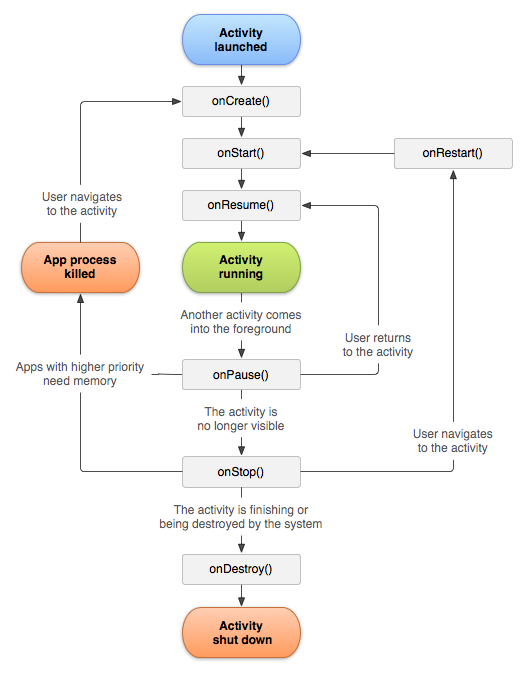
\includegraphics[width=0.33\textwidth]{img/modelle/AndroidZustandsmodell.png}
	\caption[Android Zustandsmodell]{Android Zustandsmodell\protect\footnotemark}
	\label{figure:androidZustandsmodell}
\end{figure}
\footnotetext{http://www.javatpoint.com/images/androidimages/Android-Activity-Lifecycle.png}

Dieses Zustandsmodell ist auch anfangs einer der Nachteile von Android, da es nicht so leicht zu verstehen ist und uns einige Probleme bereitet hat. Nachdem wir uns aber im Laufe der App-Entwicklung immer mehr mit Android vertraut gemacht haben, war auch das Modell kein Problem mehr, sondern im Gegenteil sehr angenehm, da es sehr logisch und gut durchdacht ist. Eine weitere Schwierigkeit, die während der Entwicklung auftrat, ist die Vielzahl an verschiedenen Android-Versionen und Geräten. Da wir unsere App für so viele Versionen wie möglichen entwickeln wollten, kamen auch einige Probleme auf. Beispielsweise sind manche Libraries oder Frameworks erst ab einer bestimmten Android-Version verfügbar, und die vielen verschiedenen Geräte haben meist unterschiedliche Displaygrößen und Seitenverhältnisse.\\
Die Vorteile von Android überwiegen aber unserer Meinung nach, vor allem, nachdem man sich damit tiefer beschäftigt und sich eingearbeitet hat. Einer der größten Vorteile ist die sehr gute Dokumentation von Android, wodurch das Einlesen in die Möglichkeiten und Funktionen recht leicht ist. Auch die weltweite Verbreitung und Beliebtheit von Android ist hier ein Vorteil, da es sehr viele Entwickler gibt und so jedes Problem schon einmal aufgetreten ist und daher auch meist schon Lösungen oder Hilfestellungen verfügbar sind.

Außerdem wird Android stetig Weiterentwickelt, weshalb immer mehr möglich ist und der Umgang mit bestimmten Funktionen, wie etwa der Zugriff auf Gerätefunktionen wie Kamera oder Galerie, immer leichter wird. Weitere Vorteile für uns sind die Vertrautheit mit Java und die Einfachheit der eigens von Google bereitgestellten Entwicklungsumgebung, ``Android Studio''.

% Abschnitt: Frameworks
\section{Frameworks}
\label{sec:grundlagen:frameworks}
Frameworks sind Ansammlungen von Funktionen, die wiederverwendet werden können um einen gezielten Bereich der Implementierung zu erleichtern und die Anzahl an neu zu implementierenden Funktionen zu verringern.\\
Wir haben in unserer App drei Frameworks als Hilfen genutzt:
\begin{itemize}
\item Picasso\footnote{http://square.github.io/picasso/}: Erlaubt einen wesentlich einfacheren Umgang hinsichtlich Anzeige, (asynchronem) Laden, und Transformation von Bildern.
\item MPAndroidCharts\footnote{https://github.com/PhilJay/MPAndroidChart}: Ermöglicht die Erstellung von Diagrammen - in unserem Fall Kuchendiagramme zur Visualisierung der Statistiken
\item Floating Action Button / Floating Action Menu\footnote{https://github.com/Clans/FloatingActionButton}: Eine Erweiterung des standardmäßigen Floating Action Buttons in Form eines Menüs, das ein- und ausgeklappt werden kann.
\end{itemize}




















\newcommand{\reqtable}[3]{
    \begin{center}
    \begin{tabular}{ | l | p{13cm} |}
    \hline
    \textbf{ID:} & \textbf{#1} \\ \hline
    TITEL: & #2 \\ \hline
    BES: & #3 \\
    \hline
    \end{tabular}
    \end{center}
}

\chapter{Anforderungsanalyse}	
\label{cha:anforderungsanalyse}
In diesem Kapitel werden die ursprünglich definierten funktionalen und nichtfunktionalen Anforderungen tabellarisch dargestellt. Jede der Anforderungen hat einen eindeutigen Identifikator (ID), einen Titel (TITEL), und eine Beschreibung (BES).

% Abschnitt: Funktionale Anforderungen
\section{Funktionale Anforderungen}
\label{sec:anforderungsanalyse:funktional}

\reqtable{FA1}{Startmenü}{Nach dem Start der Anwendung sieht der Benutzer ein Startmenü mit den Einträgen „Spiel starten“, „Einstellungen“, „Spielregeln“, „Deckübersicht“ („Rangliste“), („Infos“)}
\reqtable{FA2}{Einstellungen}{Es gibt eine Möglichkeit, die Spieleinstellungen zu ändern. Diese umfassen Schwierigkeitsgrad, Soundeffekte (an/aus) und Spielmodus (rundenbasiert/zeitbasiert/Kartenbasiert)}
\reqtable{FA3}{Spielregeln}{Es gibt eine Möglichkeit, die Spielregeln anzuzeigen.}
\reqtable{FA4}{Infoseite}{Es gibt eine Möglichkeit, eine Infoseite (mit Copyright- und weiteren Informationen) anzuzeigen}
\reqtable{FA5}{Deckübersicht}{Der Benutzer hat die Möglichkeit eine Liste mit allen verfügbaren Decks anzuzeigen. Beim Auswählen eines Decks kann der Benutzer durch die Karten des Decks scrollen. Dabei sieht er bei jeder Karte das Bild und die Attribute. Außerdem kann der Benutzer auf der Deckübersichts-Seite neue Decks hinzufügen. Diese Decks dienen als „Erweiterung“ und der Benutzer kann sie sich herunterladen.}
\reqtable{FA6}{Spiel starten}{Der Benutzer hat vom Startmenü aus die Möglichkeit, das Spiel zu starten. Dafür öffnet sich ein Dialog, auf dem der Benutzer das Deck auswählt und festlegt, ob er gegen einen anderen Spieler oder gegen einen Computer spielen will. Danach werden die Karten auf die beiden Spieler verteilt und es wird zufällig bestimmt, welcher Spieler beginnt.}
\reqtable{FA7}{Spielablauf}{Während des Spiels sieht der Spieler pro Runde nur seine „oberste Karte im Stapel“. In einer Runde werden die Werte des erstgewählten Attributs verglichen. Nach Auswahl eines Attributs vom ersten Spieler werden die zu vergleichenden Werte beider Spieler angezeigt und das gewinnende Attribut markiert. Bei einem Gleichstand werden die Karten beider Spieler unter den jeweils eigenen Stapel gelegt.}
\reqtable{FA8}{Spielstand anzeigen}{Während des Spiels wird dauerhaft der Spielstand (Anzahl Karten Spieler 1 : Anzahl Karten Spieler 2) angezeigt.}
\reqtable{FA9}{Spielzeit anzeigen}{Beim zeitbasierten Modus wird neben dem Spielstand auch die verbleibende Rundenzeit und die verbleibende Gesamt-Spielzeit angezeigt.}
\reqtable{FA10}{Spielende}{Das Spiel ist vorbei, wenn
\begin{itemize}
\item {[alle Modi]} ein Spieler alle Karten hat (Dieser Spieler hat gewonnen)
\item {[Zeitbasiert]} die Zeit abgelaufen ist (Der Spieler mit den meisten Karten hat gewonnen)
\item {[Rundenbasiert]} die vorher ausgewählte Anzahl an Runden gespielt worden sind (Spieler mit den meisten Karten hat gewonnen)
\end{itemize}
}
\reqtable{FA11}{Speicherung der Daten}{Die Daten des Spiels (Decks, Karten und ihre Attribute) werden in einer Datenbank gespeichert. Dabei gilt für jedes Deck:
\begin{itemize}
\item Die Anzahl an Karten soll eine gerade Zahl zwischen 16 und 64 sein.
\item Die Anzahl an Attributen soll eine Zahl zwischen 5 und 10 sein.
\item Für jedes Attribut wird spezifiziert, ob ein höherer Wert oder ein niedriger Wert gewinnt.
\end{itemize}
}

% Abschnitt: Nichtfunktionale Anforderungen
\section{Nichtfunktionale Anforderungen}
\label{sec:anforderungsanalyse:nichtfunktional}

\reqtable{NFA1}{Entwicklungssprache und -Umgebung}{Die Anwendung wird in Java mit der Entwicklungsumgebung „Android Studio“ entwickelt und soll auf Geräten mit Betriebssystemen ab Android [4.1] funktionieren.}
\reqtable{NFA2}{Reaktionszeit}{Die Reaktionszeit der Anwendung soll zu jeder Zeit maximal 1,5 Sekunden betragen}
\reqtable{NFA3}{Persistenter Spielzustand}{Während eines Spiels soll die App minimiert werden können (z.B. durch den Home Button), ohne dass der Spielzustand verloren geht. D.h., ein Spiel soll bei erneutem Öffnen fortgesetzt werden können.}
\reqtable{NFA4}{Benutzbarkeit}{Die Anwendung soll intuitiv bedienbar sein. D.h., die Buttons und andere Auswahlmöglichkeiten sollen eine ausreichende Größe haben und wie erwartet reagieren.}
\reqtable{NFA5}{Offline-Modus}{Die Anwendung soll stets auch das Spielen ohne Internetanbindung ermöglichen.}
\chapter{Konzept und Entwurf}

Wie üblich bei einem Projekt startet man mit Mockups der Anwendung, damit der Kunde eine genauere Vorstellung seiner Ideen bekommt. 

Wir haben uns ziemlich stark an unsere Mockups gehalten und im Folgenden sieht man jedes Mockup gepaart mit dem dazugehörigen Screenshot aus der fertigen App.

Wenn man die App öffnet befindet man sich als erstes auf der Startseite.\\

\begin{figure}[h]
    \centering
    \begin{minipage}{0.45\textwidth}
        \centering
        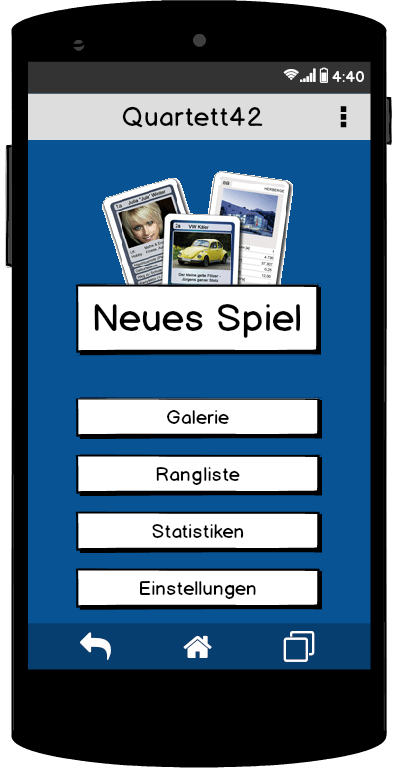
\includegraphics[width=0.75\textwidth]{img/mockups/main_screen.png}
        \caption{first figure}
    \end{minipage}
    \begin{minipage}{0.45\textwidth}
        \centering
        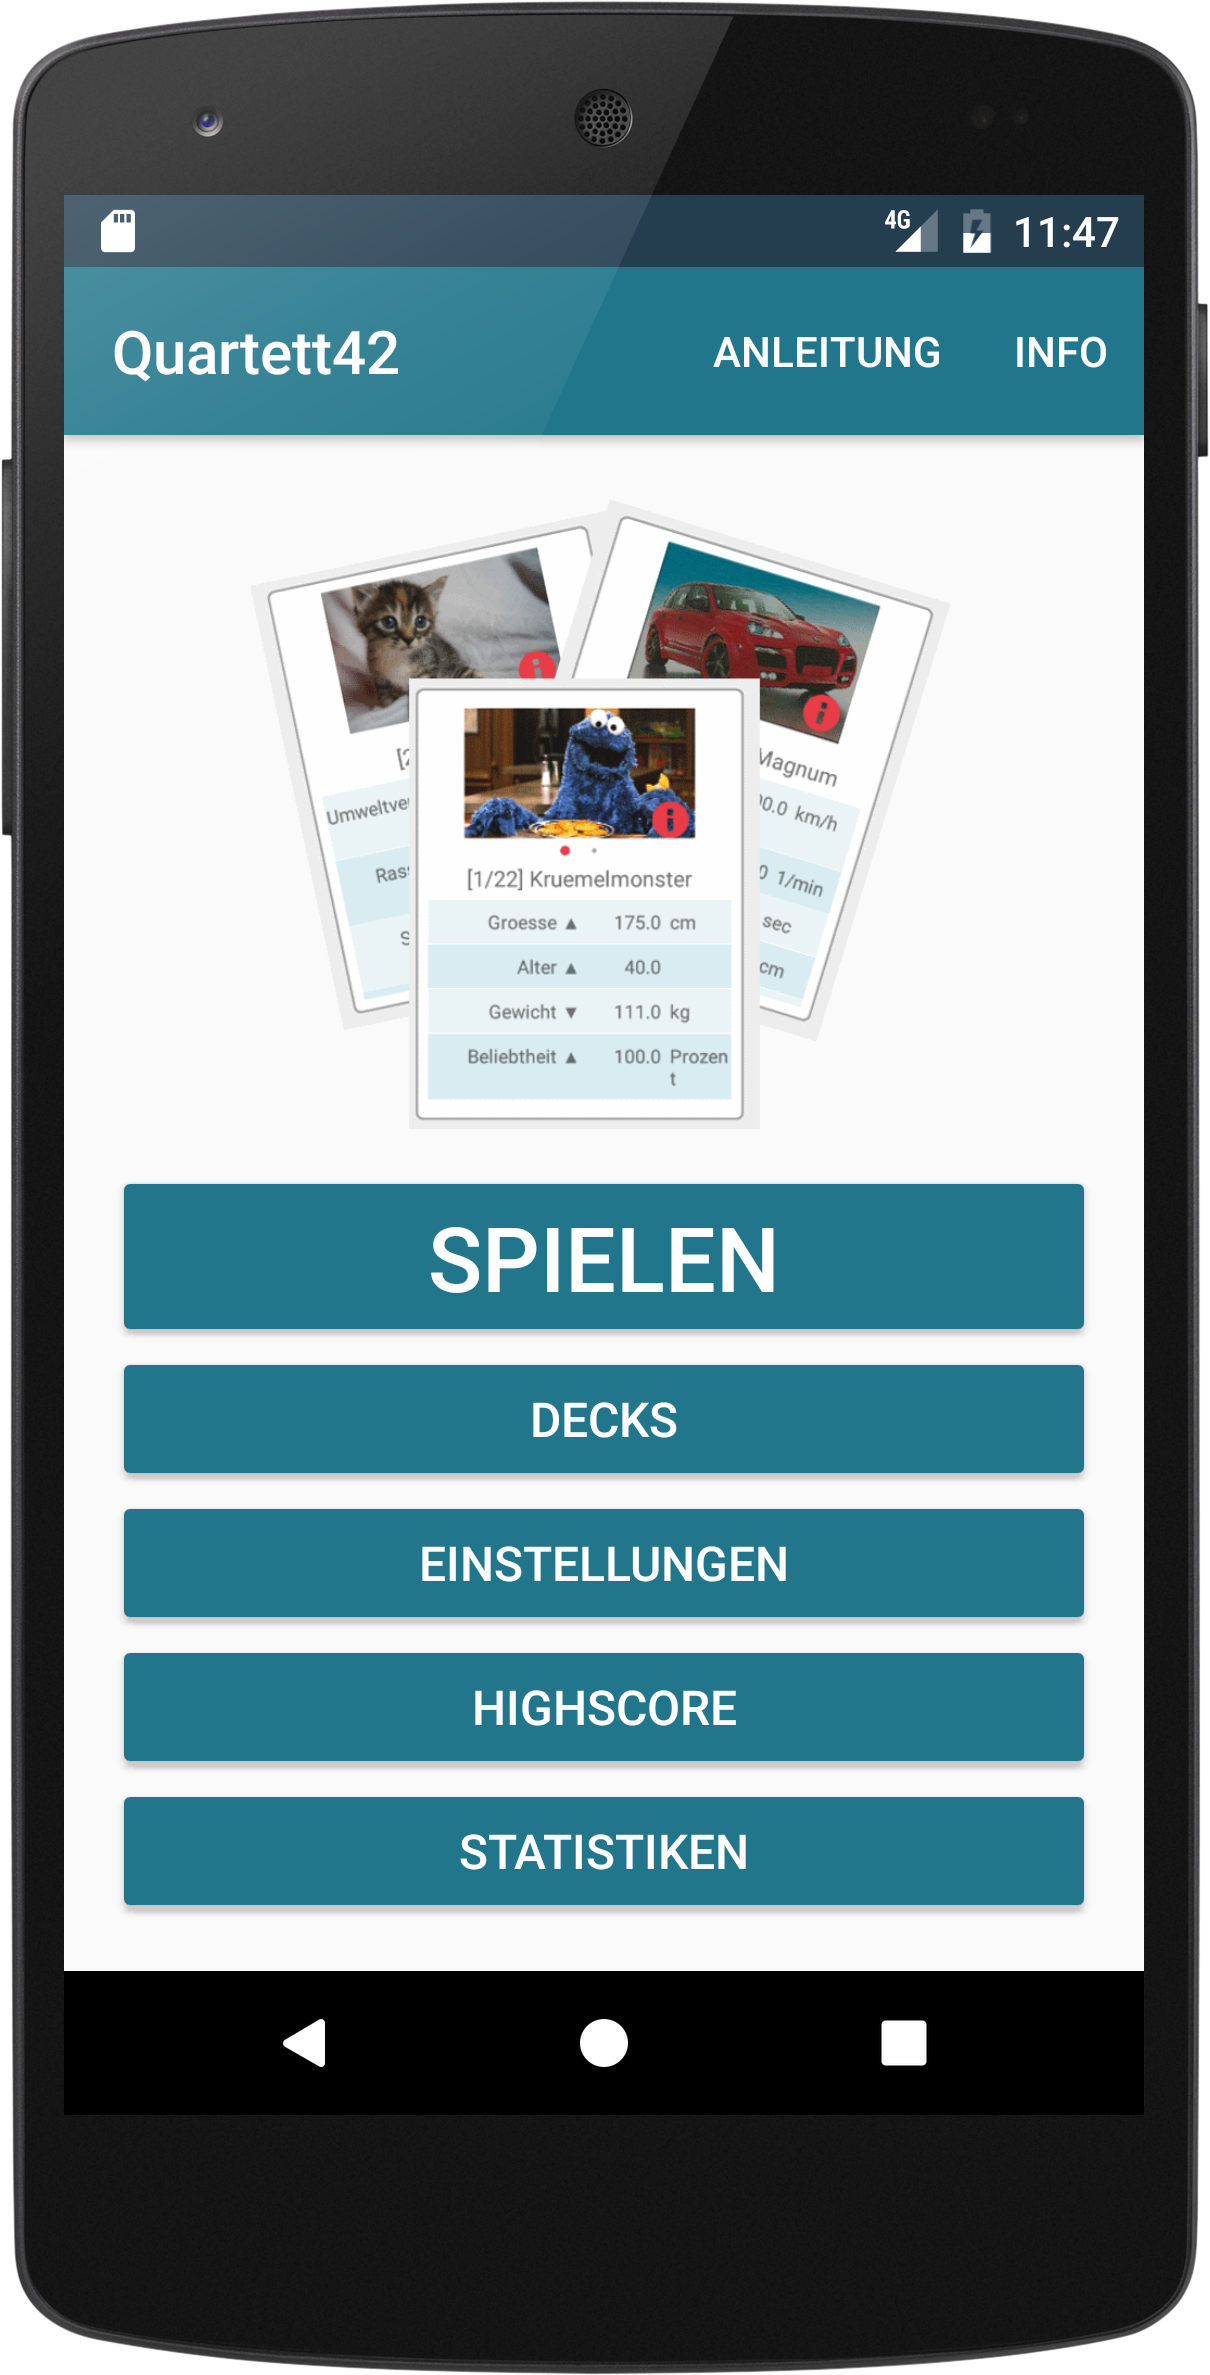
\includegraphics[width=0.75\textwidth]{img/screenshots/device_main_screen.png}
        \caption{second figure}
    \end{minipage}
\end{figure}

Als nächstes manövriert man zu einem neuen Spiel. Hier haben wir, anders als in dem Mockup, die Einstellungen nur angezeigt, aber man kann sie natürlch noch ändern bevor man das Spiel startet. Ein Deck muss aber jedes mal gewählt werden. \\

\begin{figure}[h]
    \centering
    \begin{minipage}{0.45\textwidth}
        \centering
        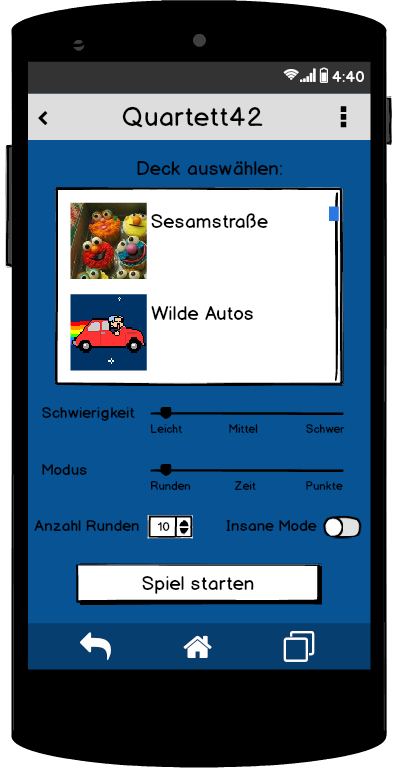
\includegraphics[width=0.4\textwidth]{img/mockups/neues_spiel.png}
        \caption{first figure}
    \end{minipage}\hfill
    \begin{minipage}{0.45\textwidth}
        \centering
        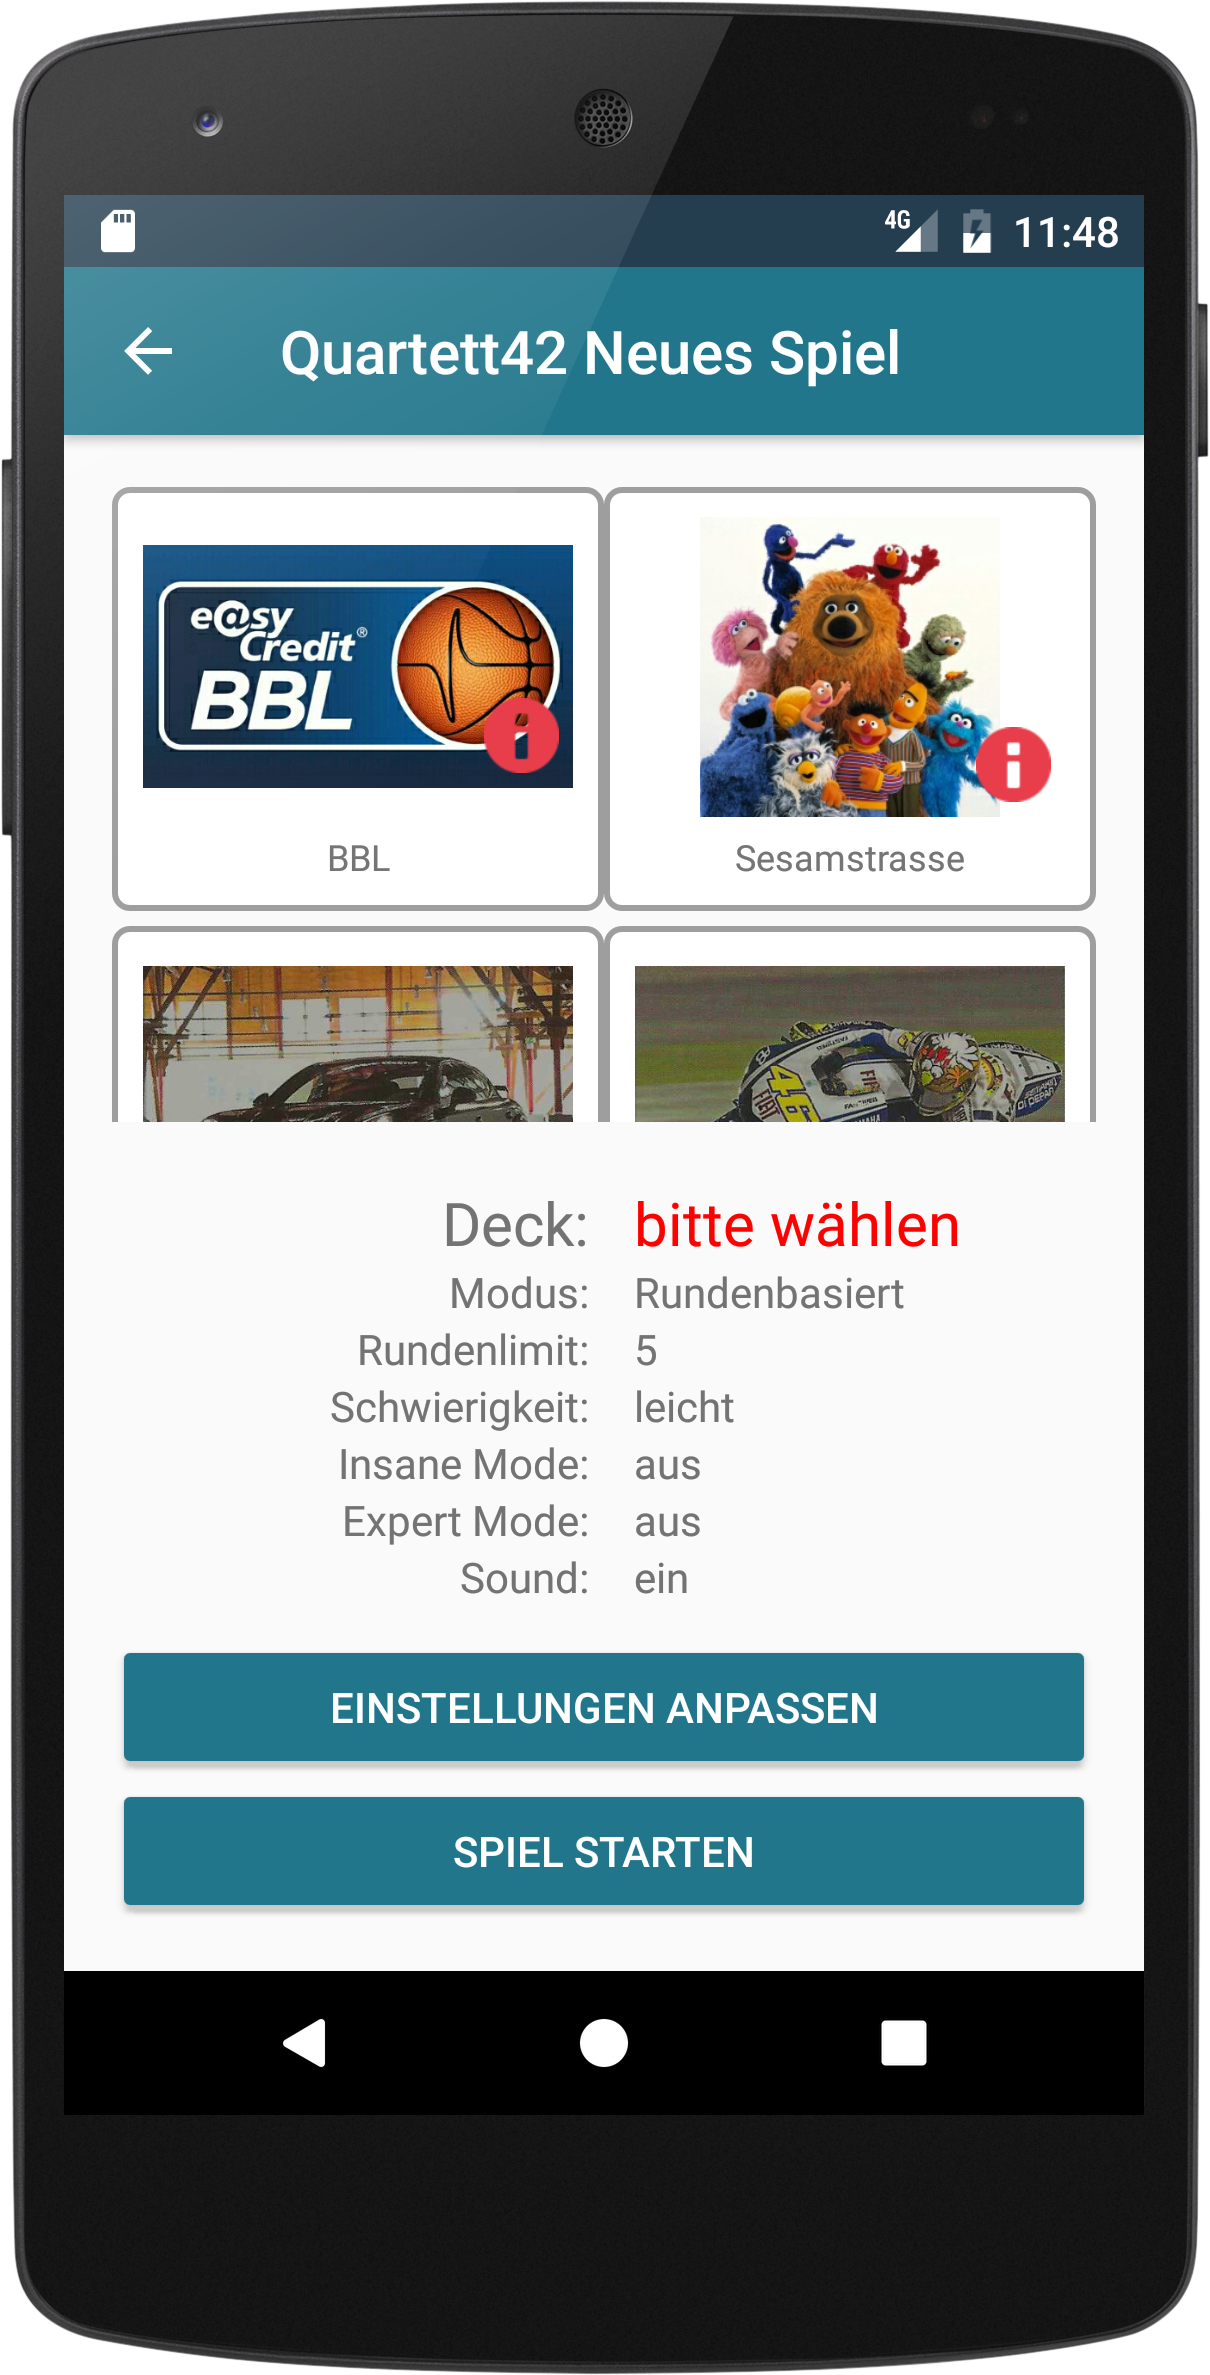
\includegraphics[width=0.4\textwidth]{img/screenshots/device_new_game.png}
        \caption{second figure}
    \end{minipage}
\end{figure}

Will man jetzt doch noch etwas an den Einstellungen ändern, tippt man auf Einstellungen anpassen und kann nun beliebig Anpassungen vornehmen.

\begin{figure}[h]
    \centering
    \begin{minipage}{0.45\textwidth}
        \centering
        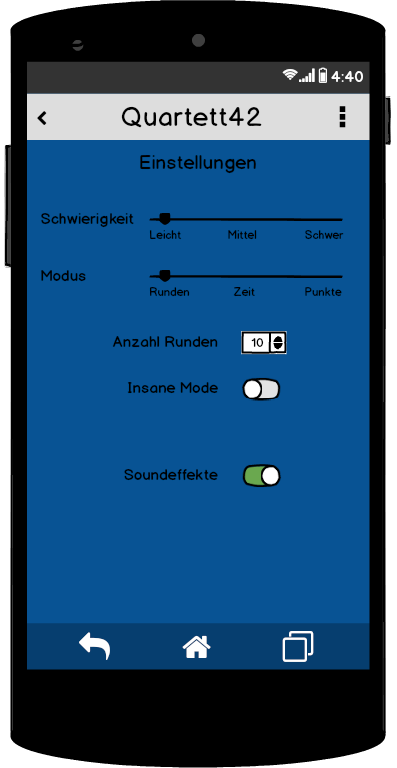
\includegraphics[width=0.4\textwidth]{img/mockups/einstellungen.png}
        \caption{first figure}
    \end{minipage}\hfill
    \begin{minipage}{0.45\textwidth}
        \centering
        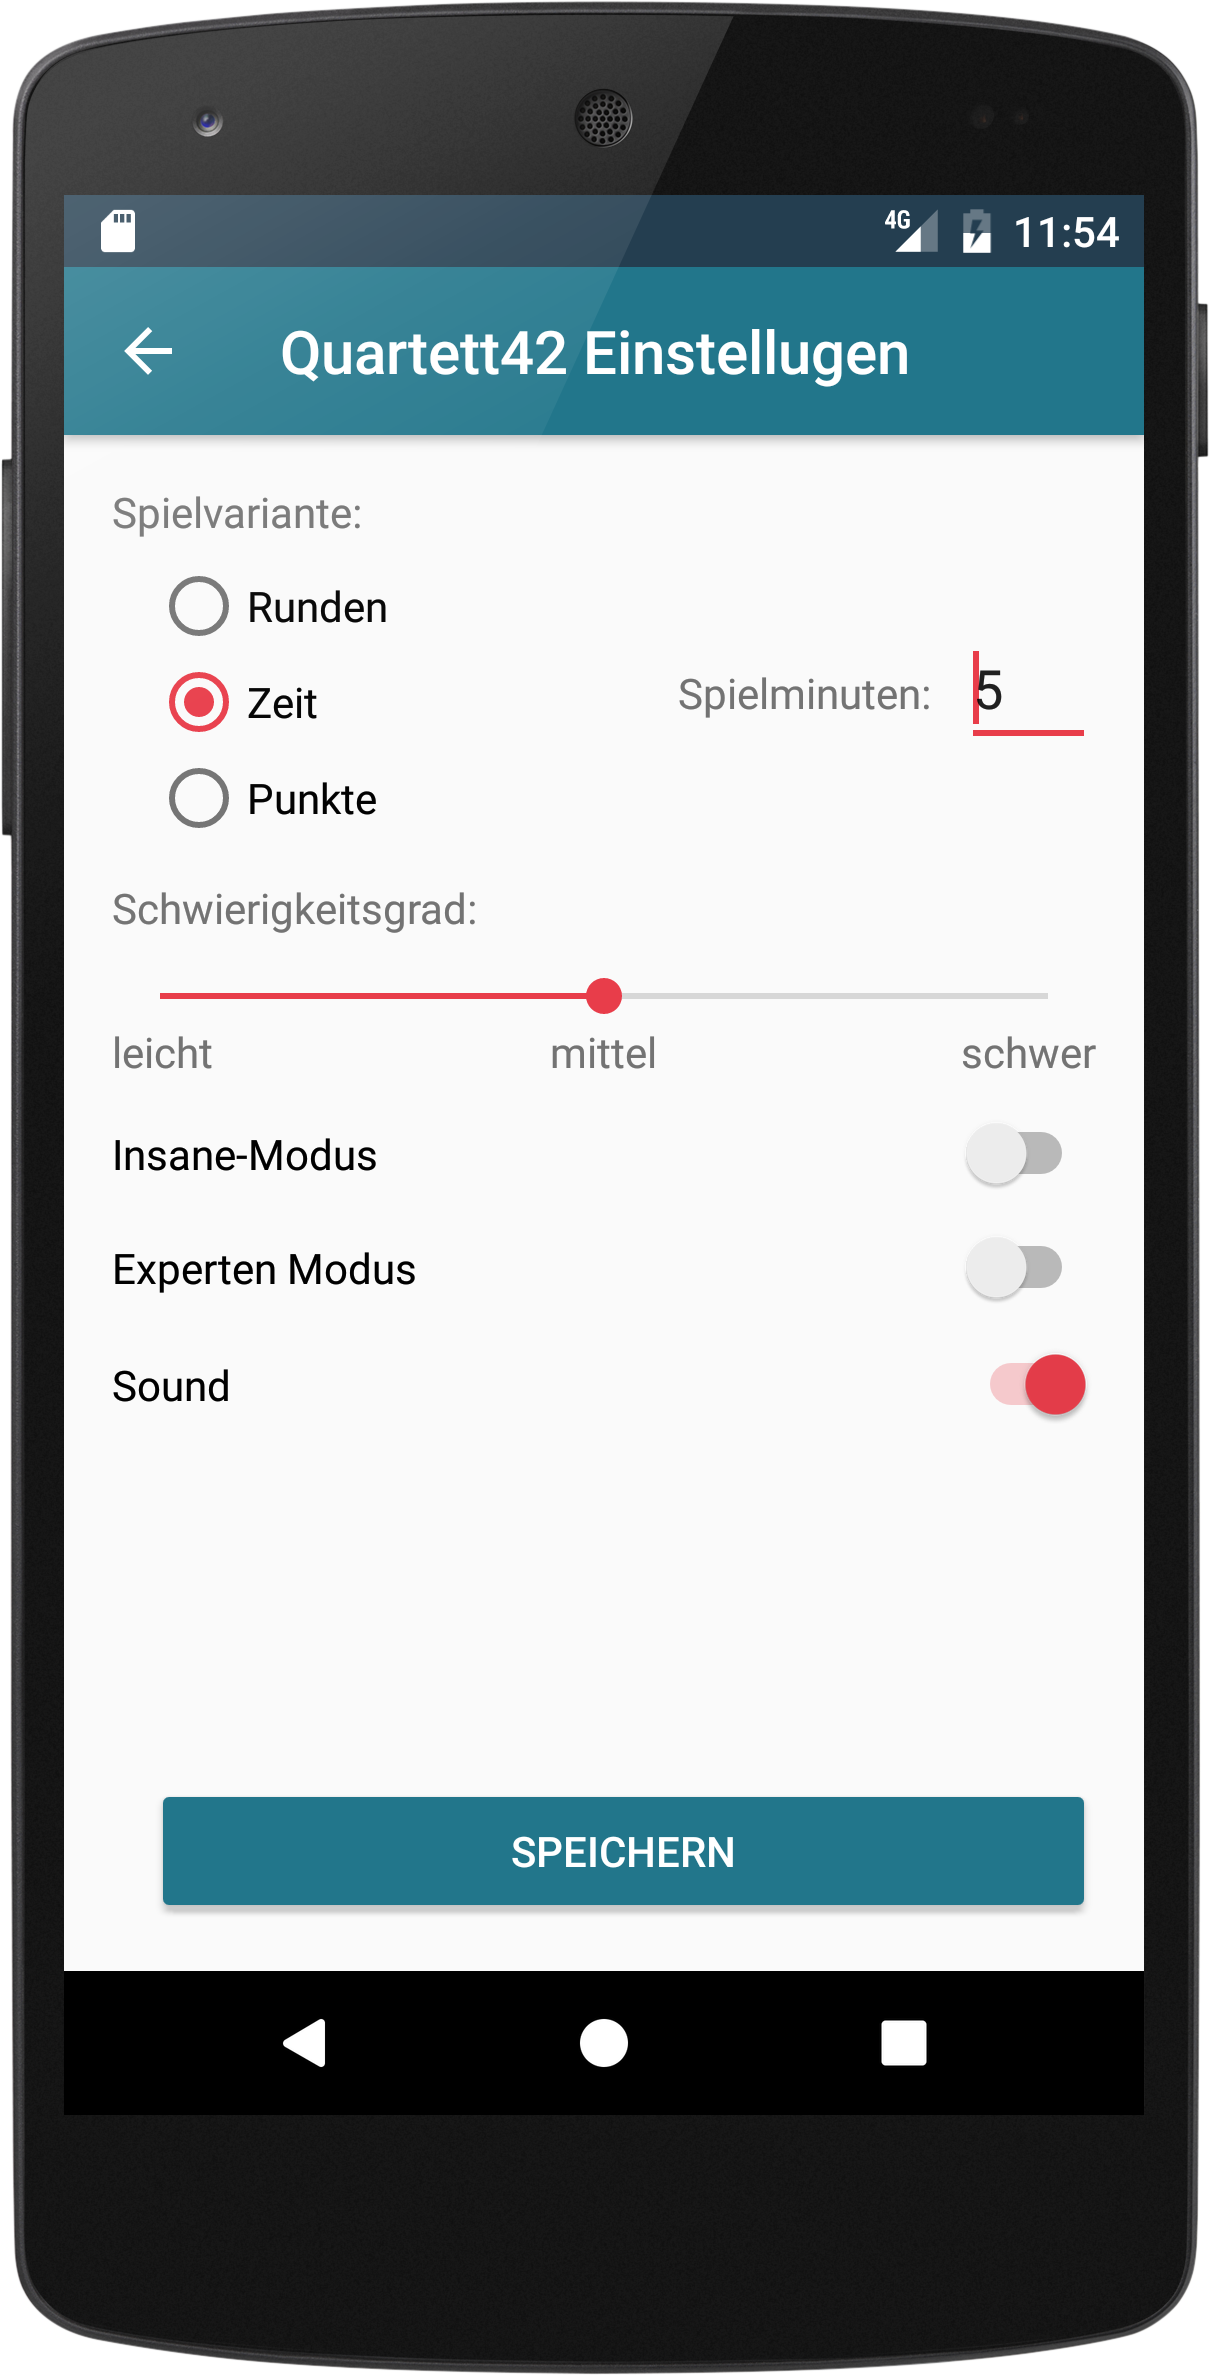
\includegraphics[width=0.4\textwidth]{img/screenshots/device_settings.png}
        \caption{second figure}
    \end{minipage}
\end{figure}

\chapter{Implementierung}
\label{cha:implementierung}

blablabla

% Abschnitt: Implementierungsdetails
\section{Implementierungsdetails}
\label{sec:implementierung:implementierungsdetails}

- keine Ahnung was da am besten bei uns erklärt werden kann
- Algorithmen: möglichwerweise die "KI" oder die Punkteberechnung
- vielleicht Galerie-Darstellung durch Grid-Layout-Adapter?

% Abschnitt: Architektur
\section{Architektur}
\label{sec:implementierung:architektur}

- ein paar Einleitungssätze
- Datenmodell aus Präsentation kopieren und erlüutern, was besonders ist (auf Speicherung mit JSON eingehen)
- Klassen-/Activity-Modell aus Präsentation kopieren
- Download- und Upload-Verlauf-Modell (muss noch erstellt werden)
- vielleicht ein paar Sätze zu allgemeinem Vorgehen und Aufteilung??

% Abschnitt: Besonderheiten 
\section{Besonderheiten}
\label{sec:implementierung:besonderheiten }	

- Deckcreator und -editor vorstellen
- Up- und Download von Decks
- ...

% Abschnitt: Schwierigkeiten während der Implementierung 
\section{Schwierigkeiten während der Implementierung}
\label{sec:implementierung:schwierigkeiten }	

Wie in Präsentation
\chapter{Anforderungsabgleich}
\label{cha:anforderungsabgleich}

% Abschnitt: Funktionale Anforderungen
\section{Funktionale Anforderungen}
\label{sec:anforderungsabgleich:funktional}


% Abschnitt: Nicht Funktionale Anforderungen
\section{Nicht Funktionale Anforderungen}
\label{sec:anforderungsabgleich:nichtfunktional}
\chapter{Zusammenfassung und Ausblick}
\label{cha:zusammenfassungUndAusblick}

- Zusammenfassung: gute App geworden und wir haben viel gelernt ...
- Ausblick was die App angeht: App eigentlich fertig aber könnte an manchen Stellen noch optimiert werden (Design, weitere Funktionen,...)
- Ausblick was das Team angeht: erlerntes Wissen in das Entwickeln neuer Apps umsetzen

% Bibliograhpy
\bibliographystyle{splncs}
\begingroup
\interlinepenalty 10000
\sloppy
\bibliography{literature}
\endgroup

% anhänge
\appendix
% hier kommen die anhänge
\chapter{Quelltexte}

In diesem Anhang sind einige wichtige Quelltexte aufgeführt.

\begin{lstlisting}[caption={Zeilencode}]
public class Hello {
    public static void main(String[] args) {
        System.out.println("Hello World");
    }
}
\end{lstlisting}


\backmatter			% abtrennung für verzeichnisse

% hier die verzeichnisse
\listoffigures
%\listoftables


\clearpage
%\erklaerung

\end{document}
